\documentclass[12pt,letterpaper]{article}
\usepackage{fullpage}
\usepackage[top=0.25cm, bottom=3.25cm, left=1cm, right=1cm]{geometry}
\usepackage{amsmath,amsthm,amsfonts,amssymb,amscd}
\usepackage{enumerate}
\usepackage{fancyhdr}

% Graphis options
\usepackage{graphicx}
\usepackage{wrapfig}
\usepackage{caption}
\usepackage{subcaption}
\graphicspath{ {./image/} }
% Code options
%\usepackage[T1]{fontenc}
%\usepackage[scaled=0.9]{FiraMono}
%\usepackage{listings}
%\lstset{basicstyle=\ttfamily}


\setlength{\parindent}{0.0in}
\setlength{\parskip}{0.05in}

\pagestyle{fancyplain}
\headheight 35pt
\lhead{Melaney (Yuanyuan) Zhu \\ 1006879255}
\chead{\textbf{\Large ProbQuiz}}
\rhead{CSC384 \\ \today }
\rfoot{\small\thepage}
\headsep 1.5em

\begin{document}

\section*{Bayes' Burrito}


\paragraph{(a) How many different types of burrito bowls are there}  \mbox{}\\

For each type of rice, it can be paired with 4 types of beans; In terms of the topping combination, the customer would be able to choose any subset of the 7 topping options. Therefore the total number of choices for toppings would be: $2^{7}$. Combine it together

\begin{align*}
    \text{Total} &= 2 \times 4 \times 2^{7} \\
                 &= 8 \times 128 \\
                 &= 1024
\end{align*}

Therefore, there are 1024 different types of burrito bowls possible.


\paragraph{(b) Eshan's burrito bowl}  \mbox{}\\

The factorization goes as follows: 

$$ P_{Eshan}(R, B, T) = P(R) \times  P(B) \times P(T \mid R, B) $$

\begin{itemize}
    \item $P(R)$: need 1 independent value (2 possibilities, knowing 1 would imply the other, since the possibilities must sum up to 1)
    \item $P(B)$: need 3 independent values (similar reason as above)
    \item $P(T \mid R, B)$: firstly there are 2 options for $R$, 4 options for $B$, and $2^{7}$ options for $T$, therefore for each combination of $R, B$, need $(2^{7} - 1)$ independent values; lastly calculate the conditional probability for $P(T \mid R, B) = 2 \times 4 \times (2^{7} - 1) = 1016$
\end{itemize}

Putting them tougher, the total number of independent values needed to know is $1 + 3 + 1016  = 1020$. Thus, 1020 values must be known to fully compute $P_{Eshan}(R, B, T)$.


\paragraph{(c) Zafeer's burrito bowl}  \mbox{}\\

The factorization goes as follows: 

$$ P_{Zafeer}(R, B, T) = P(R) \times  P(B \mid R) \times P(T) $$

\begin{itemize}
    \item $P(R)$: need 1 independent value (2 possibilities, knowing 1 would imply the other, since the possibilities must sum up to 1)
    \item $P(B)$: for each types of rice, have 4 options, but 3 needs calculation (they sum up to 1), therefore the independent values for this conditional probability is $2 \times 3 = 6$ 
    \item $P(T \mid R, B)$: need $2^{7} - 1 = 127$ independent values (same reason as above)
\end{itemize}

Putting them tougher, the total number of independent values needed to know is $1 + 6 + 127  = 134$. Thus, 134 values must be known to fully compute $P_{Zafeer}(R, B, T)$.


\section*{Bayesian Network}

% \begin{figure}[h]
%     \caption{}
%     \centering
%     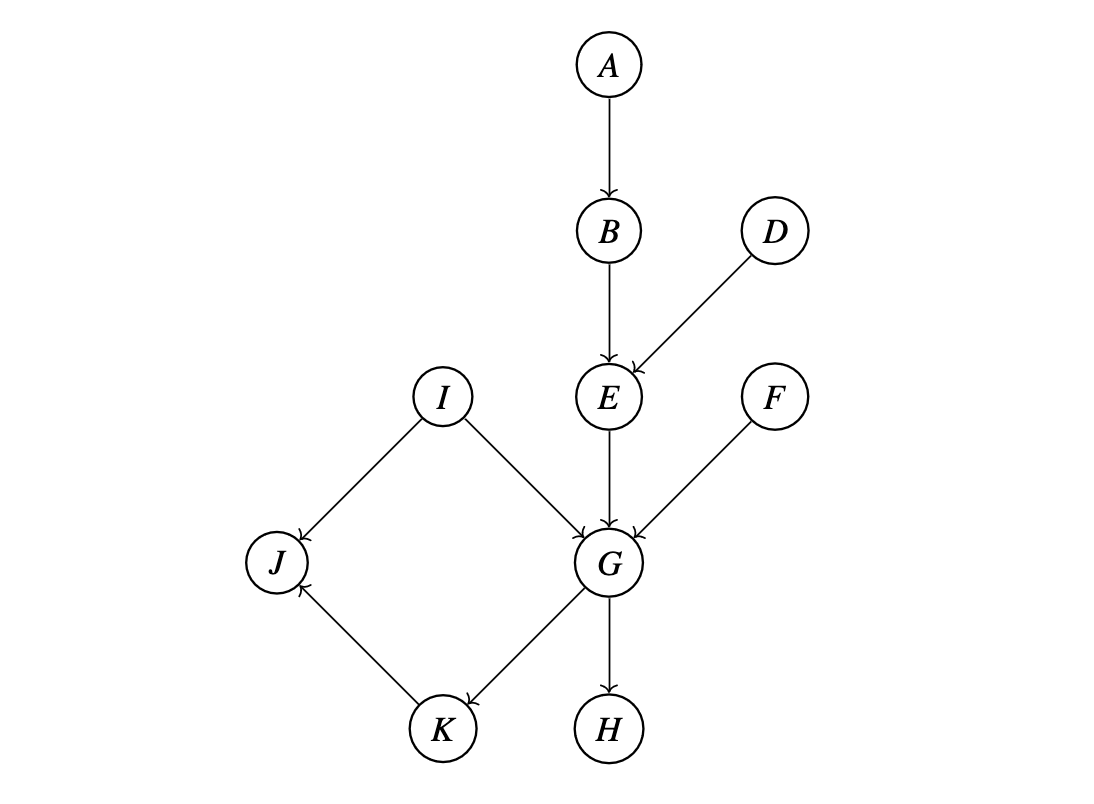
\includegraphics[width=0.3\textwidth]{example_net}
%     \label{}
% \end{figure}

\paragraph{(a) Variables independent of $I$}  \mbox{}\\

Variables $A, B, E, D, F$ are independent of $I$

\begin{itemize}
    \item $A, B, E$ because they are not ancestors or descendants of $I$, and no path from $I$ to them
    \item $D, F$ because it is not connected to $I$ and does not share common descendants with $I$
\end{itemize}

\paragraph{(b) Variables that are conditionally independent of $A$ given $K$}  \mbox{}\\

Given $K$, $A$ is conditionally independent of $J, I, D, F$

\begin{itemize}
    \item $J$ because conditioning on $K$ block the path from $A$ to $J$ through $K$, conditioning on $K$ makes $J$ d-separated from $A$
    \item $I, D, F$ because there are no path connecting $A$ to $D$ or $F$, regardless $K$ is conditioned or not
\end{itemize}

\paragraph{(c) Variables that are conditionally independent of $B$ given $E$}  \mbox{}\\

Given $E$, $B$ is conditionally independent of $D, I, F$

\begin{itemize}
    \item $D$ because it is a non descendant of $B$ and does not have any influence that has not already being accounted for by $E$
    \item $I, F$ because there are no path connecting $B$ to $I, F$, regardless $E$ is conditioned or not
\end{itemize}

% \newpage 

\section*{Drawing a Bayesian Network}

\begin{figure}[h]
    \centering
    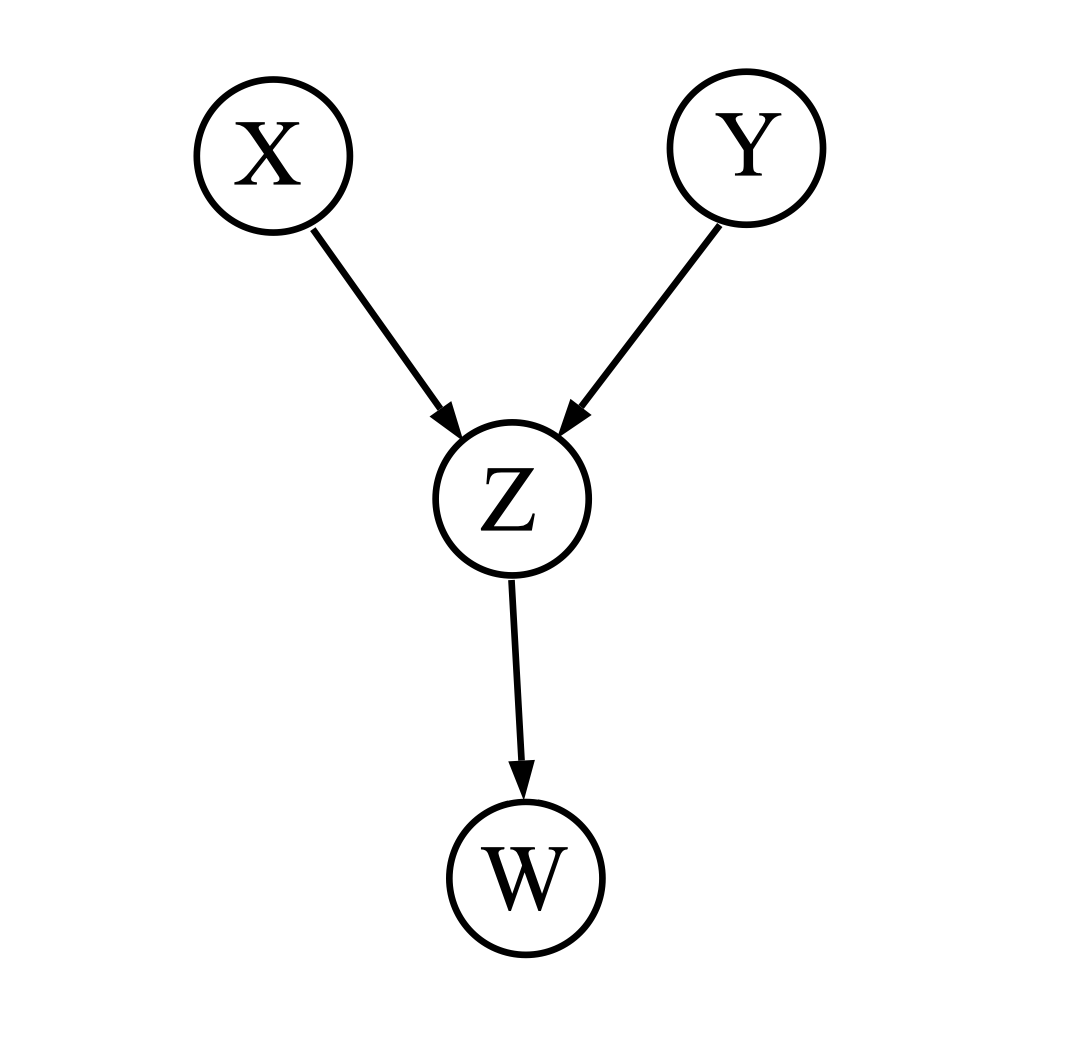
\includegraphics[width=0.3\textwidth]{my_network}
\end{figure}

$Z$ as the common effect of $X, Y$, satisfying the condition that $X, Y$ are conditionally independent given $Z$. When $X, Y$ are both known, $Z, W$ becomes conditionally independent, because $X, Y$ already contains all the information for $Z$, along with any information that $Z$ will provide for $W$.

\section*{Amazing Race Problem}

\paragraph{(a) Calculate all $M, N$ for $P(F = yes \mid N, M)$}  \mbox{}\\

First, consider that there are 2 choices for $M: \left\{ train, car \right\}$ and 3 choices for $N : \left\{ 0, 1, 2 \right\}$. Therefore there are 6 possible combinations for making the flight, below it will be calculated separately.

\subsection{$M = train, N = 0$}

\begin{align*}
    P(yes \mid 0, train) = \quad &P(yes \mid early, fast) \cdot P(early \mid train, 0) \cdot P(fast \mid 0) \\
                                &+ P(yes \mid early, slow) \cdot P(early \mid train, 0) \cdot P(slow \mid 0) \\
                                &+ P(yes \mid late, fast) \cdot P(late \mid train, 0) \cdot P(fast \mid 0) \\
                                &+ P(yes \mid late, slow) \cdot P(late \mid train, 0) \cdot P(fast \mid 0) \\
    = \quad &(0.95 \cdot 0.9 \cdot 0.9) \quad + \quad (0.7 \cdot 0.9 \cdot [1-0.9]) \quad + \quad (0.7 \cdot [1-0.9] \cdot 0.9) \\
            &+ (0.35 \cdot [1-0.9] \cdot [1-0.9]) \\
    = \quad &0.7695 \quad + \quad 0.063 \quad + \quad 0.063 \quad + \quad 0.0035 \\
    = \quad &0.899
\end{align*}

\subsection{$M = train, N = 1$}

\begin{align*}
    P(yes \mid 1, train) = \quad &P(yes \mid early, fast) \cdot P(early \mid train, 1) \cdot P(fast \mid 1) \\
                                &+ P(yes \mid early, slow) \cdot P(early \mid train, 1) \cdot P(slow \mid 1) \\
                                &+ P(yes \mid late, fast) \cdot P(late \mid train, 1) \cdot P(fast \mid 1) \\
                                &+ P(yes \mid late, slow) \cdot P(late \mid train, 1) \cdot P(fast \mid 1) \\
    = \quad &(0.95 \cdot 0.85 \cdot 0.8) \quad + \quad (0.7 \cdot 0.85 \cdot [1-0.8]) \quad + \quad (0.7 \cdot [1-0.85] \cdot 0.8) \\
            &+ (0.35 \cdot [1-0.85] \cdot [1-0.8]) \\
    = \quad &0.646 \quad + \quad 0.119 \quad + \quad 0.084 \quad + \quad 0.0105 \\
    = \quad &0.8595
\end{align*}

\subsection{$M = train, N = 2$}

\begin{align*}
    P(yes \mid 2, train) = \quad &P(yes \mid early, fast) \cdot P(early \mid train, 2) \cdot P(fast \mid 2) \\
                                &+ P(yes \mid early, slow) \cdot P(early \mid train, 2) \cdot P(slow \mid 2) \\
                                &+ P(yes \mid late, fast) \cdot P(late \mid train, 2) \cdot P(fast \mid 2) \\
                                &+ P(yes \mid late, slow) \cdot P(late \mid train, 2) \cdot P(fast \mid 2) \\
    = \quad &(0.95 \cdot 0.6 \cdot 0.7) \quad + \quad (0.7 \cdot 0.6 \cdot [1-0.7]) \quad + \quad (0.7 \cdot [1-0.6] \cdot 0.7) \\
            &+ (0.35 \cdot [1-0.6] \cdot [1-0.7]) \\
    = \quad &0.399 \quad + \quad 0.126 \quad + \quad 0.196 \quad + \quad 0.042 \\
    = \quad &0.763
\end{align*}

\subsection{$M = car, N = 0$}

\begin{align*}
    P(yes \mid 0, car) = \quad &P(yes \mid early, fast) \cdot P(early \mid car, 0) \cdot P(fast \mid 0) \\
                                &+ P(yes \mid early, slow) \cdot P(early \mid car, 0) \cdot P(slow \mid 0) \\
                                &+ P(yes \mid late, fast) \cdot P(late \mid car, 0) \cdot P(fast \mid 0) \\
                                &+ P(yes \mid late, slow) \cdot P(late \mid car, 0) \cdot P(fast \mid 0) \\
    = \quad &(0.95 \cdot 0.75 \cdot 0.9) \quad + \quad (0.7 \cdot 0.75 \cdot [1-0.9]) \quad + \quad (0.7 \cdot [1-0.75] \cdot 0.9) \\
            &+ (0.35 \cdot [1-0.75] \cdot [1-0.9]) \\
    = \quad &0.6375 \quad + \quad 0.0525 \quad + \quad 0.1575 \quad + \quad 0.00875 \\
    = \quad &0.85625
\end{align*}

\subsection{$M = car, N = 1$}

\begin{align*}
    P(yes \mid 1, car) = \quad &P(yes \mid early, fast) \cdot P(early \mid car, 1) \cdot P(fast \mid 1) \\
                                &+ P(yes \mid early, slow) \cdot P(early \mid car, 1) \cdot P(slow \mid 1) \\
                                &+ P(yes \mid late, fast) \cdot P(late \mid car, 1) \cdot P(fast \mid 1) \\
                                &+ P(yes \mid late, slow) \cdot P(late \mid car, 1) \cdot P(fast \mid 1) \\
    = \quad &(0.95 \cdot 0.75 \cdot 0.8) \quad + \quad (0.7 \cdot 0.75 \cdot [1-0.8]) \quad + \quad (0.7 \cdot [1-0.75] \cdot 0.8) \\
            &+ (0.35 \cdot [1-0.75] \cdot [1-0.8]) \\
    = \quad &0.57 \quad + \quad 0.105 \quad + \quad 0.14 \quad + \quad 0.0175 \\
    = \quad &0.8325
\end{align*}

\subsection{$M = car, N = 2$}

\begin{align*}
    P(yes \mid 2, car) = \quad &P(yes \mid early, fast) \cdot P(early \mid car, 2) \cdot P(fast \mid 2) \\
                                &+ P(yes \mid early, slow) \cdot P(early \mid car, 2) \cdot P(slow \mid 2) \\
                                &+ P(yes \mid late, fast) \cdot P(late \mid car, 2) \cdot P(fast \mid 2) \\
                                &+ P(yes \mid late, slow) \cdot P(late \mid car, 2) \cdot P(fast \mid 2) \\
    = \quad &(0.95 \cdot 0.75 \cdot 0.7) \quad + \quad (0.7 \cdot 0.75 \cdot [1-0.7]) \quad + \quad (0.7 \cdot [1-0.75] \cdot 0.7) \\
            &+ (0.35 \cdot [1-0.75] \cdot [1-0.7]) \\
    = \quad &0.49875 \quad + \quad 0.1575 \quad + \quad 0.1225 \quad + \quad 0.02625 \\
    = \quad &0.805
\end{align*}

\paragraph{(b) Maximize chance to making the flight}  \mbox{}\\

Based on all 6 possibilities calculated above, it seems that choosing to go to the airport by \textbf{train} and bring \textbf{0 bags} will produce the maximized change of making the flight: $89.9\%$. 

\end{document}
